\chapter{Introduction}
\section{Motivation}
Humankind has only a few ways to generate reliable, non-intermittent baseload 
power: fossil fuels, hydropower, geothermal power, and nuclear energy. 
Because of increasing global climate change concerns, sources with negligible 
CO$_2$ footprints are crucial measures for global temperature control. Thus, 
from an environmental viewpoint, hydro and nuclear power are preferable ways 
to generate reliable power. However,  local geographical conditions limit the 
potential for hydropower; hence, the only option left is nuclear power. 
Nuclear power plants provided 10\% of the global electricity supply in 2018 
\cite{iea_nuclear_2019}. Moreover, nuclear share in energy generation is 
projected to stay constant through 2040, while electricity demand will 
increase by 30\% \cite{noauthor_world_2017}. This work pushes simulation tools 
with the potential to advance this vital option.

The Generation IV International Forum (GIF) chose \glspl{MSR} among the six 
advanced reactor concepts for further research and development. \glspl{MSR} 
offer significant improvements ``in the four broad areas of sustainability, 
economics, safety and reliability, and proliferation resistance and physical 
protection" \cite{doe_technology_2002}. To achieve the goals formulated by the 
GIF, \glspl{MSR} simplify the reactor core and improve inherent safety by 
using liquid coolant, which is also a fuel\footnote{Herein \glspl{MSR} are 
assumed to be reactors with liquid fuel, which simultaneously serves as a 
coolant.}. In a thermal spectrum \gls{MSR}, liquid fuel consists of carrier 
salt (i.e., LiF, LiF-BeF$_2$, or LiF-NaF-KF) and fluorides of fissile and/or 
fertile materials (i.e., UF$_4$, PuF$_3$ and/or ThF$_4$). The fuel salt 
circulates in a loop-type primary circuit \cite{haubenreich_experience_1970}. 
This innovation leads to immediate advantages over traditional, solid-fueled 
reactors. These include near-atmospheric pressure in the primary loop, 
relatively high coolant temperature, outstanding neutron economy, a high level 
of inherent safety, reduced fuel preprocessing, and the ability to 
continuously remove fission products and add fissile and/or fertile elements 
without shutdown \cite{leblanc_molten_2010}. The possibility of continuously 
removing neutron poisons increases the potential fuel burnup and thus 
improves the resource utilization of \glspl{MSR}. Finally, \glspl{MSR} 
also could be employed for the transmutation of spent fuel from current 
\glspl{LWR} \cite{fratoni_design_2004}.

Recently, interest in \glspl{MSR} has resurged, with multiple new companies 
pursuing commercialization of \gls{MSR} designs both domestically and 
internationally\footnote{Examples include liquid-fueled \gls{MSR} designs from 
Terrapower, Terrestrial, ThorCon, Flibe, Copenhagen Atomics, Elysium, etc.}. 
China's \gls{MSR} program was initiated in 2011 and promises to start up a  
2MW$_{th}$ liquid-fueled test \gls{MSR} in 2020, a 10MW$_{th}$ demonstration 
reactor in 2025, and a gigawatt-level 
commercial reactor in 2050 \cite{zhang_review_2018}. The European 
Union funds the Safety Assessment of the Molten Salt Fast Reactor 
(SAMOFAR) project, in which several European research institutes and 
universities are developing various molten salt reactor prototypes 
such as the \gls{MSFR} \cite{fiorina_molten_2013} and the \gls{MOSART} 
\cite{ignatiev_molten_2014}. To advance these \gls{MSR} concepts, particularly 
concerning their strategies for online reprocessing and refueling, we need 
computational analysis methods capturing their unique reactor 
physics, fuel reprocessing mechanics, and chemistry.

The context of the Ph.D. dissertation is the development and assessment of an 
advanced neutronics tool for fuel depletion calculations in circulating-fuel 
nuclear reactors. The present work introduces the open-source reprocessing 
simulation package, SaltProc \cite{rykhlevskii_arfc/saltproc_2018}, which 
couples with the continuous-energy Monte Carlo depletion calculation code, 
Serpent 2 \cite{leppanen_serpent_2014}, for fuel composition dynamics analysis 
in various \glspl{MSR} taking into account a realistic, physics-driven
model of an online fuel reprocessing system.

\section{Fuel burnup and online reprocessing}\label{sec:litreview}
All liquid-fueled \gls{MSR} designs involve various levels of online fuel 
processing. Minimally, noble gaseous fission products (e.g., Kr, Xe) 
escape from the fuel salt during routine reactor operation and must be 
captured. Other systems might be used to enhance the removal of those 
elements. Most designs also call for the removal of rare earth metals from 
the core since these metals act as neutron poisons. Some designs suggest a 
more elaborate list of elements to process (Figure~\ref{fig:periodic_tab}), 
including the temporary removal of protactinium from the salt or other 
regulation of the actinide inventory in the fuel salt 
\cite{ahmad_neutronics_2015}. Fresh fuel salt with dissolved fissile and/or 
fertile material (e.g., $^{233}$U, $^{232}$Th, \gls{LEU}, a transuranic 
vector from \gls{LWR} \gls{SNF}) make up the salt mass loss caused by poison 
removal and conserves the total mass in the primary loop.
\begin{figure}[htp!] % replace 't' with 'b' to 
	\centering
	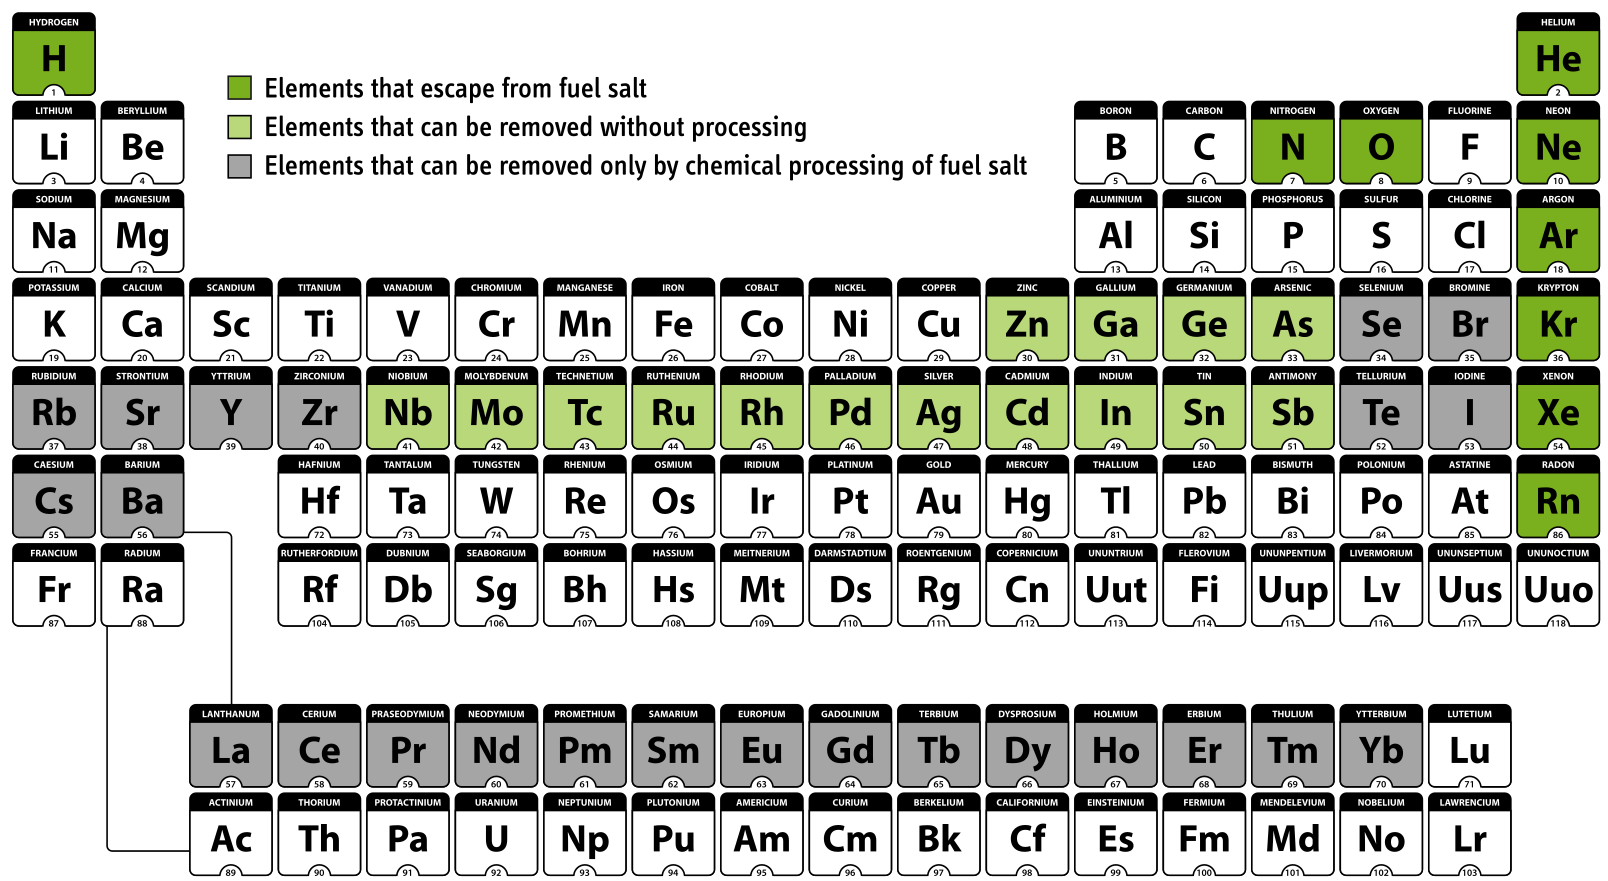
\includegraphics[width=\textwidth]{intr/periodic_map.png}
	\caption{Processing options for \gls{MSR} fuels (reproduced from 
		Ahmed \emph{et al.} \cite{ahmad_neutronics_2015}).}
	\label{fig:periodic_tab}
\end{figure}

Most liquid-fueled nuclear reactor concepts adopt continuous separations 
and feeds: the core material is circulated to or from the core at all times 
(continuously) or specific intervals (batch-wise). In contrast, in a 
solid-fueled reactor, fission products and actinides remain within the initial 
fuel material throughout its time in the core.

The ability to perform online fuel salt reprocessing improves the potential 
neutronics performance of liquid-fueled reactors. First, liquid-fueled 
reactors can operate with relatively low excess reactivity because fissile 
material can be continuously added to the core. Second, continuously removing 
fission products, including strong absorbers (poisons), can significantly 
improve fuel utilization and decrease parasitic neutron absorption. Third, 
online reprocessing decreases the amount of decay heat, dissipating after 
shutdown. Finally, for a breeder\footnote{\gls{CR} 
	$\equiv$ fissile generated/fissile consumed: if CR $<$ 1, the reactor is a 
	``converter''; CR $\equiv$ 1, an ``isobreeder''; CR $>$ 1, a 
	``breeder.''} excess of fissile material might be continuously extracted  
from the core and used to startup new reactors. Nevertheless, the removal of
each element from the liquid fuel salt presents a unique challenge in terms of
chemical separation, storage, and disposal of the separated materials.

Contemporary nuclear fuel depletion software lacks continuous fuel salt 
reprocessing modeling. To handle material flows in potential online removal 
and feed of liquid-fueled systems, early \gls{MSR} simulation methods at 
\gls{ORNL} integrated neutronics and fuel cycle codes (i.e., Reactor Optimum 
Design (ROD) \cite{bauman_rod_1971}) into operational plant tools (i.e., 
Multiregion Processing Plant (MRPP) \cite{kee_mrpp_1976}) for \gls{MSR} fuel 
reprocessing system design. Extensive research in fast and thermal MSR 
analysis has yielded specialized tools for burnup calculations in 
liquid-fueled nuclear systems \cite{fiorina_investigation_2013, 
sheu_depletion_2013, aufiero_extended_2013, heuer_towards_2014, 
park_whole_2015, betzler_molten_2017, betzler_molten_2019}. 
Table~\ref{tab:msr_codes} presents a list of recent efforts, along with the 
main features of the employed methods and software.
\FloatBarrier

\begin{table}[htbp]
	\fontsize{9}{11}\selectfont
	\caption{Tools and methods for liquid-fueled \gls{MSR} fuel salt 	
	depletion analysis.}
	\begin{tabularx}{\textwidth}{p{0.13\textwidth} p{0.18\textwidth} 	
	p{0.18\textwidth} p{0.15\textwidth} p{0.2\textwidth}} 
	\hline
	&Nuttin \emph{et al.}, 2005 \cite{nuttin_potential_2005}& Aufiero 
	\emph{et al.}, 2013 \cite{aufiero_extended_2013} & Betzler \emph{et al.}, 
	2018 \cite{betzler_fuel_2018}&Present work \\ \hline
	Neutronics&\gls{MCNP}&Serpent 2 &SCALE6.2     &Serpent 2 \\
	software  & REM      &          &ORIGEN-S     &			       \\
         	  &stochastic&stochastic&deterministic&stochastic      \\[10pt]
	Geometry  & unit cell& full-core 3D&unit cell&full-core 3D\\      [10pt]
	Removal/feed  & continuous &continuous & batch-wise & batch-wise\\[10pt]
	Separation efficiency &\multicolumn{3}{c}{fixed, must be defined by 
	user before simulation} & function of many para\-me\-ters \\ [10pt]
	Fuel reprocessing plant & \multicolumn{3}{c}{single component, 	``black'' 
	box model} & realistic multi-compo\-nent model \\ [10pt]
	Reactivity control & \multicolumn{2}{c}{continuous adjustment of fissile 
	material injection} & batch injection of fissile material & periodical 
		adjustment of geometry and fissile material injection\\ [10pt]
	Safety parameters evolution & thermal feedback & not considered & thermal 
	feedback & thermal feedback, control rod worth, axial offset \\
	\hline
	\end{tabularx}
	\label{tab:msr_codes}
\end{table}

Two main online reprocessing simulation approaches have been demonstrated in 
the literature: batch-wise and continuous. In the batch-wise approach, the 
burnup simulation stops at a given time and restarts with a new liquid fuel 
composition (after removal of discarded materials and addition of 
fissile/fertile materials). 

\gls{ORNL} researchers have developed ChemTriton, a Python script for
SCALE/TRITON, which employs the batch-wise approach to simulate a continuous 
reprocessing and refill for either single or multiple fluid designs.  
ChemTriton models salt treatment, separations, discharge, and refill using  
SCALE/TRITON depletion simulation over small time steps to simulate continuous 
reprocessing and deplete the fuel salt \cite{betzler_fuel_2018, 
powers_new_2013}.

In the continuous approach, accounting for removal or addition of material 
presents a greater challenge since it requires adding a term to the Bateman 
equations. Both ORIGEN \cite{gauld_isotopic_2011} and the Serpent burnup 
routine \cite{leppanen_burnup_2009} solves a set of the Bateman equations 
using one-group averaged flux and transmutation cross sections obtained from a 
transport calculation. The Bateman equations describe the rate of change of 
each isotope, $i$, due to neutron induced reactions and decay processes
\cite{tsoulfanidis_nuclear_2013}:
\begin{align} \label{eq:bateman}
	\frac{dN_i}{dt} &= \sum_{m=1}^{M}l_{im}\lambda_mN_m + 
	\phi\sum_{m=1}^{M}f_{im}\sigma_mN_m - (\lambda_i + \phi\sigma_i + r_i - 
	f_i)N_i + F_i\Big|{i\in [1,M]}\\
	& \qquad (1) \qquad\qquad\qquad (2) \qquad\qquad(3) \quad (4)  \quad 
	(5) \quad (6)
	\nonumber
	\intertext{where}
	N_i &= \mbox{number density of nuclide \emph{i} $[cm^{-3}]$} \nonumber \\
	M &= \mbox{number of nuclides $[-]$} \nonumber \\
	l_{im} &= \mbox{fraction of decays of nuclide \emph{m} that result in 
	formation of nuclide \emph{i} $[-]$} \nonumber \\
	\lambda_i &= \mbox{radioactive decay constant of nuclide \emph{i} 
	$[s^{-1}]$} 
	\nonumber \\
	\phi &= \mbox{neutron flux, averaged over position and energy 
	$[cm^{-2}s^{-1}]$} \nonumber \\
	f_{im} &= \mbox{fraction of neutron absorption by nuclide \emph{m} 
	leading to the formation of nuclide \emph{i} $[-]$} \nonumber \\
	\sigma_m &= \mbox{average neutron absorption cross section of nuclide 
	\emph{m} $[cm^2]$} \nonumber \\
	r_i &= \mbox{continuous removal rate of nuclide \emph{i} from the 
	system $[s^{-1}]$} \nonumber \\
	f_i &= \mbox{continuous feed rate of nuclide \emph{i} $[s^{-1}]$} 
	\nonumber \\
	F_i &= \mbox{production rate of nuclide \emph{i} directly from 
	fission $[cm^{-3}\cdot s^{-1}]$.}\nonumber
\end{align}
The terms on the right-hand side of the equation represent:
\begin{enumerate}[label=(\arabic*)]
	\item production of species $i$ as a result of the decay of all the 
	nuclides present;
	\item production of species $i$ as a result of neutron capture by all 
	nuclides present;
	\item loss of nuclide $i$ through its own decay;
	\item loss of nuclide $i$ as a result of neutron capture;
	\item loss of nuclide $i$ through continuous removal from the system;
	\item gain of nuclide $i$ as a result of continuous feed to the 
	system.
\end{enumerate} 

Nuttin \emph{et al.} developed an in-house depletion code called \gls{REM}, 
which directly couples with \gls{MCNP} \cite{werner_mcnp_2017-1} to simulate 
fuel salt material evolution in a simplified \gls{MSBR}-like liquid-fueled 
system. That work directly integrated the Bateman differential equations using 
neutron flux from \gls{MCNP}, tracking all the isotopes available in the 
data library, and controlling reactivity to maintain reactor criticality
\cite{nuttin_potential_2005}.

In a similar vein, Aufiero \emph{et al.} extended Serpent 2 for continuous 
reprocessing simulations by adding an explicit pseudo-decay term representing 
fission product removal ($-N_i r_i$ term in Equation~\ref{eq:bateman}) for 
each target poisonous nuclide \cite{aufiero_extended_2013}. The developed 
extension directly accounts for the effects of online fuel reprocessing on 
depletion calculations and features a reactivity control algorithm. The 
extended version of Serpent 2 was assessed against a dedicated version of the 
deterministic ERANOS-based EQL3D procedure in 
\cite{fiorina_investigation_2013} and applied to analyze the \gls{MSFR} fuel 
salt isotopic evolution.

More recently, Betzler \emph{et al.} added to SCALE/TRITON continuous removals 
capability for depletion simulation \cite{betzler_molten_2019}. Similar to 
Aufiero \emph{et al.} this extended SCALE/TRITON directly adds feed and 
removal terms in the burnup matrix and solves it using existing ORIGEN 
capabilities. TRITON's continuous reprocessing capability was validated 
against the batch-wise script ChemTriton for single-channel \gls{MSRE}-like 
model. Unlike ChemTriton, this new capability will be available for all SCALE 
users in the 6.3 release. However, at the moment, it is undergoing extensive 
testing and validation procedures and unavailable for external users.

Some of the tools listed in Table~\ref{tab:msr_codes} used significant  
approximations that may lead to inaccurate fuel evolution predictions and 
others unavailable for external users. This work introduces an 
open-source simulation package, SaltProc, which expands the capability of the 
continuous-energy Monte Carlo Burnup calculation code, Serpent 2, for 
depletion calculations of liquid-fueled \glspl{MSR}.

Most of the existing tools in the literature represented the fuel salt 
reprocessing plant as an invariable ``black box'' model, which removes target 
elements all at once with a fixed efficiency, determined by the user before 
starting the depletion simulation. Typically, such a ``black box'' model is 
characterized by a vector of removing elements and their extraction 
efficiencies:
\begin{align}
&\qquad\qquad\qquad\qquad
\begin{bmatrix}
N^{b}_{0} \\ \vdots \\ N^{b}_{e} \\ \vdots \\ N^{b}_{E} \\
\end{bmatrix} 
\times
\begin{bmatrix}
\epsilon_{0} \\ \vdots \\ \epsilon_{e} \\ \vdots \\ \epsilon_{E} \\
\end{bmatrix} =
\begin{bmatrix}
N^{a}_{0}\\ \vdots \\ N^{a}_{e} \\ \vdots \\N^{a}_{E}  \\
\end{bmatrix} \\
\intertext{where}
N^{b} &= \mbox{number density vector before reprocessing $[cm^{-3}]$} 
\nonumber \\
N^{a} &= \mbox{number density vector after reprocessing $[cm^{-3}]$} 
\nonumber \\
\epsilon &= \mbox{extraction efficiency $[-]$ vector for all elements $e$ in 
$(0,E)$.} \nonumber
\end{align}

The main issues related to static ``black box'' model assumptions in the 
literature neglect: 
\paragraph*{Time varying extraction.} Realistically, long-term reactor 
operation will require a time-dependent extraction efficiency vector. The 
current tools treat separation efficiency as constant.
\paragraph*{The impact of operational parameters on separation efficiency.} In 
reality, the extraction efficiency depends on temperature, power level, 
current fuel salt isotopic composition, and material mass flow rate. Gas 
solubility in the salt is inversely proportional to the salt temperature; 
hence, the extraction efficiency expected to be lower for the higher 
temperature of the salt.
\paragraph*{Discrete component performance and dynamics in the multi-component 
system.} All reprocessing plant components are treated as a single ``black 
box'' component in existing simulation tools. However, the fuel salt in a 
reprocessing plant undergoes many separate components (e.g., helium bubbling, 
nickel mesh filter, etc.) that target specific elements. Some of these 
components can be connected in series, parallel, or series-parallel. The 
``black box'' model (only single process) requires extensive pre-simulation 
analytic work from the user to calculate the lumped separation efficiency 
vector before a simulation is run and cannot be adjusted during the 
simulation. Additionally, treating the processing system as a single ``black 
box'' neglects dynamics related to relative component flow rates. Finally, the 
discrete waste streams from each component are not tracked separately in 
``black box'' tools. However, this information is necessary for fuel 
reprocessing system optimization.\\

In contrast with tools listed in Table~\ref{tab:msr_codes}, SaltProc, does not 
make these approximations. SaltProc allows the user define the separation 
efficiency as a function of time or operational parameters, and is able to 
simulate multi-component fuel reprocessing system instead of ``black box''.

\section{Operational and safety parameter evolution} 
\label{sec:saf-par-literature}
In contrast with conventional solid-fueled reactors with in-core fuel 
residence averaging 4-5 years\footnote{For the typical 18-month cycle, during 
refueling personnel removing 1/3 of the fuel assemblies, re-arranging other 
assemblies, and loading fresh fuel into the core. Thus, each fuel assembly is 
kept in the core at most $3\times 18=54$ months.}, an initial \gls{MSR} fuel 
salt batch stays in the \gls{MSR} primary loop throughout the reactor 
lifetime. 
Therefore, the fuel salt accumulates \glspl{FP} not captured by the fuel 
reprocessing system as well as transuranic elements\footnote{The chemical 
elements with atomic numbers greater than uranium (92).}. Continuous fuel 
salt composition evolution has a significant influence on the neutron energy 
spectrum and, consequently, affects the reactor behavior, necessitating 
additional safety analysis.

Nuttin \emph{et al.} studied the evolution of a key safety parameter, the 
temperature reactivity feedback coefficient, estimating it for the \gls{MSBR} 
at startup and equilibrium. The temperature coefficient of reactivity 
quantified reactivity changes due to temperature increase in the core and was 
calculated in that work as:
\begin{align}\label{eq:feedback}
	&\qquad\qquad \alpha = \frac{k_{1200} - k_{900}}{\delta 
	T} \\
	\intertext{where}
	k_{900}, k_{1200}  &= \mbox{multiplication coefficients at 900K and 
		1200K $[-]$} \nonumber \\
	\delta T &= \mbox{300 $[K]$.}\nonumber
\end{align}

That work showed that the \gls{FTC} at startup and equilibrium is $-1.5$ 
and $-1.0$ $pcm/K$, respectively\footnote{ 1 pcm = 10$^{-5}\Delta 
k_{eff}/k_{eff}$}. Nuttin \emph{et al.} also reported a positive and 
time-invariant total temperature coefficient ($+0.8$ $pcm/K$) 
\cite{nuttin_potential_2005}. Recently, Park and colleagues expanded that 
approach to a full-core high-fidelity \gls{MSBR} model and estimated safety 
parameters evolution over 20 years of operation \cite{park_whole_2015}. These 
calculations showed a relatively large negative total temperature coefficient 
during the 20 year reactor operation. DUring that time, the coefficient 
magnitude weakens from $-3.21$ to $-1.41$ $pcm/K$ from startup to equilibrium, 
respectively. Additionally, that work reported a control rod worth 
deterioration from $2099pcm$ to $1970pcm$ due to neutron spectrum hardening 
during reactor operation. 

More recently, Betzler \emph{et al.} \cite{betzler_assessment_2017-1} reported 
safety parameter evolution for the \gls{TAP} \gls{MSR}: the fuel 
reactivity coefficient at \gls{BOL} and 15 years from \gls{BOL} was negative 
and decreasing slowly over the reactor lifetime (from -4.0 to -4.1 $pcm/K$ 
when temperature was perturbed from 900K to 1200K); the moderator reactivity 
coefficient was +0.43 $pcm/K$ at \gls{BOL} and -2.7 $pcm/K$ after 15 
years of operation. Overall, thermal feedback seems to be stronger in the 
\gls{TAP} reactor and deteriorates insignificantly during the reactor 
operation. Notably, the authors ignored material density change with 
temperature to simplify temperature coefficient calculation; thus, only  
Doppler broadening was taken into account. The researchers reported the total 
worth of all control rods in the \gls{TAP} core only for the startup fuel 
composition. 

The evolution of control rod worth in the \gls{TAP} has not been reported in 
the literature before. Chapter 5 of this dissertation illuminated the 
evolution of essential safety parameters (fuel, moderator, total temperature 
coefficient, control rod worth) for the \gls{TAP} \gls{MSR} at various moments 
during the reactor operation. Additionally, I investigated the impact of 
neutron poison accumulation (e.g., $^{135}$Xe) in the fuel salt during 
short-term transients (i.e., load following) on major safety characteristics 
\cite{rykhlevskii_impact_2019}.


\section{Background Summary}
State-of-the-Art software packages for depletion analysis and evolution of 
safety parameters in the liquid-fueled \gls{MSR} are reviewed in 
Section~\ref{sec:litreview}. Based on this summary, I have identified a few 
possible directions for the improvement of \gls{MSR} tools:
\paragraph*{Reproducibility/availability.}
Serpent is the only contemporary nuclear reactor physics software that can 
perform depletion calculations that can take into account online fuel salt 
reprocessing regimes. However, this built-in online reprocessing routine is 
undocumented: the discussion forum for Serpent users is the only useful 
source of information at the moment. Other mentioned tools are available for 
internal users only. These issues can be a barrier to reuse research software 
and to reproduce scientific results. Thus, a new, open-source, reproducible 
tool for fuel processing simulation would assist in the production of 
reproducible research in the area of liquid-fueled reactor modeling.
\paragraph*{Realistic fuel reprocessing system model.} 
Significant approximations in fuel reprocessing parameters deteriorate fuel 
salt composition predictions since the evolution of safety parameter accuracy 
is strongly dependent on fuel salt composition. A realistic fuel reprocessing 
system model will allow reprocessing component parameter optimization,  
increase the fidelity of fuel and waste stream composition calculations, and 
advance reprocessing system design.
\paragraph*{Variable extraction efficiency.} Most research efforts in 
the literature (except Nuttin \emph{et al.}\footnote{Nuttin \emph{et al.} 
assumed 100\% extraction efficiency for noble gases (Xe, Kr) and protactinium, 
20\% for rare earths, 5\% for semi-noble metals, and 1\% for alkaline 
elements \cite{nuttin_potential_2005}.}) assume ideal 100\% extraction 
efficiency of all removed 
elements, which stayed constant during the whole reactor lifetime. 
Realistically the efficiency is time-dependent and changes with respect to 
operational parameters: temperature, power level, salt composition, etc. Thus, 
the ability to set up dynamic separation efficiency must be added in \gls{MSR} 
simulation tools to advance depletion calculations.
\paragraph*{Reactivity control.} Reconfigurable moderator configuration in the 
\gls{TAP} core presents a challenge because of the core geometry changes with 
time. The reactivity control module, which adjusts the core geometry 
to maintain criticality, would be an exceptional capability for simulating  
new, more advanced \gls{MSR} concepts and short-term transients.
\paragraph*{Safety characteristics evolution during reactor operation.} The 
\gls{MSR} fuel salt  accumulates \glspl{FP} and transuranic elements, which 
significantly shift the neutron energy spectrum. This spectrum shift might 
worsen the core safety during operation. The impact of the fuel salt 
evolution on the \gls{MSR} safety parameters must be carefully investigated 
and reported.\\

This work aims to overcome these issues and demonstrate the tool capabilities 
for a two promising \gls{MSR} concepts.


\section{Objectives and outline of the work}
Most of the existing \gls{MSR} depletion simulators usually assume ideal  
efficiency (100\% of the target nuclide is being removed) of the neutron 
poison removal process (see Section~\ref{sec:litreview}). The main goal of 
this dissertation is to develop a generic open-source tool, SaltProc, capable 
of simulating a wide range of liquid-fueled systems --- including multi-fluid 
and multi-region designs --- and validate it against existing modeling 
efforts. Additionally, SaltProc enables poison extraction simulation based on 
a realistic physics-based fuel processing model. 

The structure of the thesis is as follows. Chapter 1 serves as a literature 
review, providing background on fuel burnup, online fuel reprocessing  
approaches, safety parameter evolution during reactor operation, and how these 
concepts have been applied to a wide range of \glspl{MSR} in the literature. 
Chapter 2 details online reprocessing modeling and the proposed computation 
tool architecture. In an attempt to avoid the pitfalls of a ``black box''  
understanding and to identify method limitations at an early stage, governing 
equations and working principles are stated and discussed. Chapter 3 presents 
equilibrium-seeking results for the \gls{MSBR} as well as essential 
operational and safety parameters for both the initial and equilibrium states.

Additionally, the benefits of continuous fission product removal for a thermal 
\gls{MSR} are evaluated at the end of chapter 3. Chapter 4 covers SaltProc 
demonstration and validation efforts with a focus on the \gls{TAP} \gls{MSR},  
taking into account adjustable moderator configuration. Chapter 5 gives the 
safety parameter overview and its evolution during the \gls{TAP} 
lifetime-long reactor operation. Moreover, the safety parameters dynamics 
during short-term transients have been evaluated at the end of chapter 5. The 
final chapter summarizes this work's contribution to the nuclear community, 
and a conclusion is offered together with an outlook for future work on the 
topic.